\documentclass[letterpaper,12pt]{book} %tipo de documento y tama~o de papel y letra

\usepackage{mystyle} %%Reemplazar por el contenido de 'mystyle.sty' en caso de no funcionar

\begin{document} %Inicio de documento
\begin{titlepage} %portada
\thispagestyle{empty} %borrar el formato de pagina linda
%\begin{flushleft} %alinear a la izq
\begin{center}

\includegraphics[scale=0.35]{logoUSM-DI.eps}
%\vfill
\end{center}
%\end{flushleft}

%\vspace{1cm} %espacio vertical , en realidad es un enter de 2 cm
\begin{center} %centrar
  {
    \begin{figure}[H]
      \centering
      
\includegraphics[width=0.4\textwidth]{logo_Phyrex8.png}
      \label{fig:Phyrex}
    \end{figure}
    \Huge Plan de Proyecto\\
    \begin{figure}[H]
      \centering
      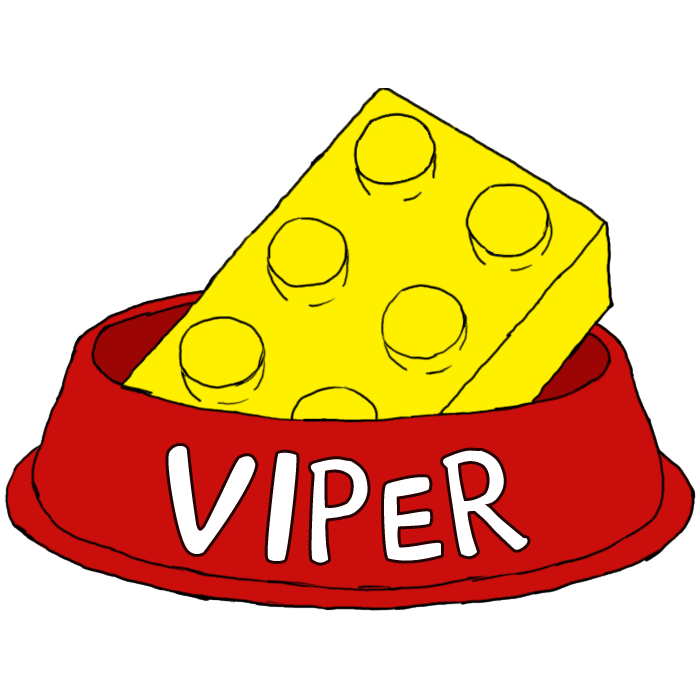
\includegraphics[width=0.2\textwidth]{VIPeR.png}
      \label{fig:Viper}
    \end{figure}
    \normalsize Santiago, 2013
  }
\end{center}

\vspace{1cm}

%\begin{figure}[H]
%  \centering
%  \begin{subfigure}[b]{0.4\textwidth}
%    \centering
%    
\includegraphics[width=\textwidth]{logo_Phyrex8.png}
%    \label{fig:Phyrex}
%  \end{subfigure}
%  ~
%  \begin{subfigure}[b]{0.25\textwidth}
%    \centering
%    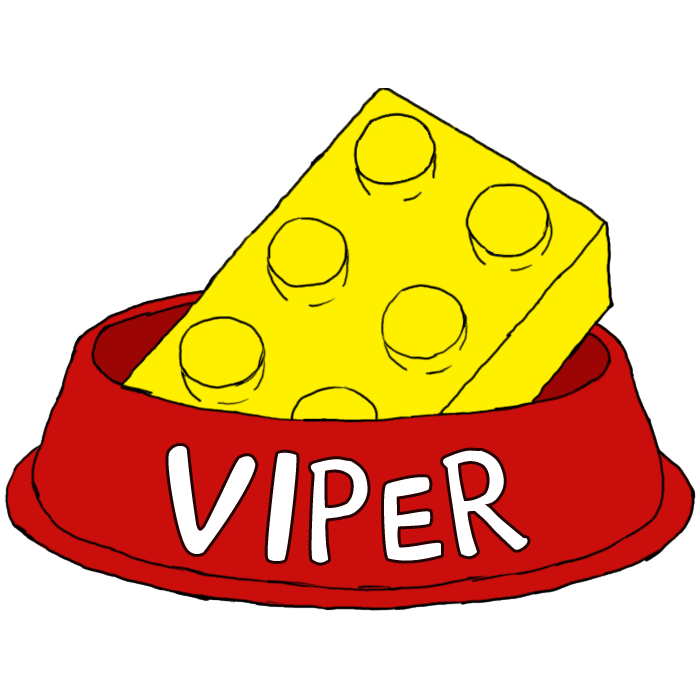
\includegraphics[width=\textwidth]{VIPeR.png}
%    \label{fig:Viper}
%  \end{subfigure}
%\end{figure}

\vfill
\begin{flushleft} %alinear izquierda
%  Pre-Empresa: \emph{Phyrex}
  Jefe de Proyecto: 
  \begin{table}[H]
    \centering
    \begin{tabular}{rll}
      Celeste Bertin     & \emph{Tel: +56 9 68410901} & \texttt{\small celeste.bertin@alumnos.usm.cl}  \\
    \end{tabular}          
  \end{table}              
  Integrantes:             
  \begin{table}[H]         
    \centering             
    \begin{tabular}{rll}   
      Rodrigo Fr\'{\i}as & \emph{Tel: +56 9 83988257} & \texttt{\small rodrigo.frias@alumnos.usm.cl}   \\
      Rocio Fernandez    & \emph{Tel: +56 9 62426549} & \texttt{\small rocio.fernandezu@alumnos.usm.cl}\\
      Juan Avalo         & \emph{Tel: +56 9 78072458} & \texttt{\small juan.avalo@alumnos.usm.cl}      \\
    \end{tabular}
  \end{table}
\end{flushleft}
\end{titlepage}

%    Patricio Carrasco &\texttt{\small <patricio.carrascod@alumnos.usm.cl>} &[+56 9 50626689]\\
 %Inclusion del titulo

\pagenumbering{Roman} %numero de paginas de indices en numeros romanos
\tableofcontents %indice de capitulos, secciones y subsecciones
\listoffigures   %indice de imagenes
\cleardoublepage
\listoftables    %indice de tablas
\cleardoublepage


%\chapter{Introducci\'on}
Uno de los grandes problemas, hoy en d\'ia, para quienes trabajan en el \'area de la inform\'atica, es el gran desconocimiento que existe en ella. Una forma de evitar esto, es el motivar a alumnos a conocer las distintas \'areas de trabajo de los que trabajan en inform\'atica. Para ello, se han realizado distintas actividades en la Universidad T\'ecnica Federico Santa Mar\'ia (UTFSM), que hacen uso de robots, para captar la atenci\'on de su p\'ublico objetivo.

\emph{Virtual Interactive Pet Robot} (en adelante denominado \emph{VIPeR}) nace como una forma de paliar el problema de motivaci\'on y desconocimiento de la labor de quienes trabajan en el \'area inform\'atica. Se enfoca, principalmente, en responder a las necesidades de nuestro cliente, adecu\'andose a los proyectos de captaci\'on de estudiantes de Ense\~nanza Media que ya existen en la UTFSM, en su campus Santiago. Para este prop\'osito, \emph{VIPeR} se enmarca dentro de una serie de actividades que utilizan el sistema LEGO Mindstorms como forma de atraer a futuros estudiantes a la inform\'atica.

En la secci\'on 2 se mostrar\'a que ideas similares existen actualmente, indicando similitudes y diferencias con la idea propuesta. Se identificar\'an las restricciones impuestas por el cliente, adem\'as de alternativas a la soluci\'on y se encontrar\'a la que mejor se ajusta a nuestros requerimientos.

En la secci\'on 3 se definir\'a el modelo de desarrollo del proyecto, adem\'as de los elementos a utilizar junto con las competencias del equipo. En la siguiente, se indicar\'an los riesgos y el plan de contingencia o de mitigaci\'on, seg\'un corresponda.

En la secci\'on 5 se muestran los planes para el funcionamiento del proyecto, su entrega y su mantenci\'on. Finalmente en la secci\'on 6 se indica la planificaci\'on de desarrollo del proyecto

\pagenumbering{arabic} %numeracion en numeros arabicos
\setcounter{page}{1} %empezar enumerando la pagina 1
\part{Parte P\'ublica}            %% Parte Publica
\chapter{Soluci\'on Conceptual.}
\newpage
\section{Diagn\'ostico de la situaci\'on actual.}
\subsection{Situaci\'on Actual.}

En la actualidad existen distintas tecnolog\'ias en cuanto a las mascotas que se est\'an desarrollando en el mundo. A pesar de ello, es posible catalogarlas en dos grandes grupos:

\begin{enumerate}
\item Mascotas Virtuales
\item Mascotas Rob\'oticas
\end{enumerate}

En cuanto a las Mascotas Virtuales, estas corresponden a aquellas que no poseen un cuerpo real con el cual interactuar y su medio de presentaci\'on corresponde a un dispositivo (dise\~nado para ese \'unico prop\'osito o para varios) que, por medio de botones o instrucciones dadas por medio de una pantalla, interact\'ua con la mascota correspondiente.

Por otro lado, las Mascotas Rob\'oticas poseen un nivel de complejidad mayor en gran medida debido a la presencia de un cuerpo f\'isico con el cual el usuario puede interactuar. La mascota no solo debe saber responder a est\'imulos distintos del entorno, sino que incluso el cuerpo mismo debe poder mostrar las reacciones correspondientes (a pesar de que esto no es necesario que ocurra con todo el cuerpo).

Finalmente, se destacan algunos productos correspondientes a ambas \'areas:
\begin{enumerate}
\item Mascotas Virtuales:
  \begin{enumerate}
  \item \emph{Pou},\footnote{\url{https://play.google.com/store/apps/details?id=me.pou.app/}} una aplicaci\'on para Android, que posee minijuegos sencillos, adem\'as de las caracter\'isticas naturales de unas mascota (como alimentarlo o ba\~narlo, por ejemplo). Tambi\'en permite la interacci\'on con las mascotas de otros usuarios.
  \item \emph{Mou},\footnote{\url{http://www.windowsphone.com/es-cl/store/app/mou/c032d62c-7f6a-4538-8150-f77034dcf335/}} aplicaci\'on de Windows Phone similar a Pou, aunque posee con una cantidad de juegos y acciones posibles, m\'as limitado que este.
  \item \emph{Tamagotchi},\footnote{\url{http://tamagotchilife.com/}} dispositivo port\'atil que simular una mascota, la cual debe cuidarse y criarse. Tambi\'en tiene la habilidad de interactuar con otros dispositivos en sus versiones m\'as recientes.
  \item \emph{Pet Society},\footnote{\url{https://www.facebook.com/petsociety/info}} conocida aplicaci\'on de Facebook en la que se cuida y juega con una mascota, adem\'as de posibilitar la interacci\'on con las mascotas de la lista de contactos del usuario que utilizan dicha aplicaci\'on.
  \item \emph{Petz},\footnote{\url{http://petz.uk.ubi.com/}} saga de juegos para las consolas Nintendo en la cual el usuario se encarga de cuidar perros y gatos, los cuales (para el caso de las consolas port\'atiles) pueden interactuar con otros.
  \end{enumerate}
\item Mascotas Rob\'oticas:
  \begin{enumerate}
  \item \emph{Furby},\footnote{\url{http://www.furby.es/es_ES/}} famosas en los 2000, los cuales era posible alimentar e interactuaban con otros de su misma clase.
  \item \emph{FurReal Friends},\footnote{\url{http://www.hasbro.com/furreal/en_US/}} mascotas rob\'oticas dise\~nadas para ni\~nas, las cuales reaccionan a caricias y realizan gestos similares a las de una mascota real.
  \item \emph{Aibo},\footnote{\url{http://www.sony-aibo.co.uk/}} mascota fabricada por Sony. Simula un perro y posee sensores que le evitan chocar con objetos, una cola que funciona como antena adem\'as de ``sentido del tacto'' y un simulador de inteligencia artificial. Es utilizado por universidades e institutos para realizar estudios de inteligencia artificial.
  \end{enumerate}
\end{enumerate}


\subsection{Identificaci\'on de problemas y deficiencias.}

Si bien el mundo de las mascotas virtuales ha tenido cambios desde sus or\'igenes, estos no han variado mucho respecto a su concepci\'on original, sino que su mayor cambio ha sido en cuanto a la forma de realizar la interacci\'on con ellos, cambio que fue potenciado con la llegada de los dispositivos Touch.

En contraparte, el aumento en el nivel de tecnolog\'ia actual, y la disminuci\'on de tama\~no de procesadores y otros componentes electr\'onicos, ha permitido la llegada al mercado de mascotas rob\'oticas a precios accesibles, situaci\'on que habr\'ia sido imposible a\~nos antes. Adem\'as de esto, las nuevas tecnolog\'ias permiten agregarle mayores funcionalidades a los robots utilizados. De esta manera puede verse una gran diferencia entre \emph{Furby}, que tan s\'olo permit\'ia la identificaci\'on de ciertos patrones de voz y el movimiento de ojos y orejas, y \emph{Aibo}, que posee sensores de sonido, inteligencia artificial y sensores t\'actiles, lo que lo convierten en una mascota m\'as realista (adem\'as de tener un movimiento similar al de un perro real).

A pesar de que ambas tecnolog\'ias han avanzado, hay que destacar que no existe una forma de interactuar entre ellas, y su utilizaci\'on actual corresponde \'unicamente a potenciar la primera o la segunda. Dicha brecha corresponde a un problema en el uso de las mascotas virtuales, ya que es una potencialidad que podr\'ia ser aprovechable a futuro.

Cabe destacar, en todo caso, que la adopci\'on masiva de mascotas rob\'oticas es un tema de discusi\'on aparte, debido a la necesidad, de estas, de poder desenvolverse eficientemente en el medio al que sea llevado, lo cual requiere un alto nivel de tecnolog\'ia, lo cual redundar\'ia en un mayor costo para el usuario.

Omitiendo lo anterior, por caer fuera de nuestro rango de acci\'on, mezclar las tecnolog\'ias actuales en rob\'otica, junto con las correspondientes en el \'area de los dispositivos m\'oviles, para utilizar ambos en el desarrollo de mascotas virtuales se destaca como una de las grandes falencias, en la actualidad, en el uso de este tipo de aplicaciones. Es un nicho no potenciado en el presente, y que podr\'ia ser de gran potencialidad, debido a la masificaci\'on que existe en estos momentos en el uso de dispositivos m\'oviles.

\newpage
\section{Caracterizaci\'on del cambio.}
\subsection{Caracter\'isticas y potencialidades deseadas.}

Se espera que el sistema a implementar posea y/o sea capaz de:
\begin{itemize}
\item {\bf Simular una mascota a trav\'es de un dispositivo m\'ovil, espec\'ificamente un smartphone, con SO Android};
\item {\bf Permitir la interacci\'on entre el usuario y la mascota virtual, por medio de los distintos elementos internos del smartphone} (como son la pantalla t\'actil, aceler\'ometro, sensor de sonido, bater\'ia, entre otros);
\item {\bf Permitir la interacci\'on entre el usuario y el robot LEGO Mindstorms, por medio de los sensores disponibles para este} y
\item {\bf Permitir la interacci\'on entre el smartphone con SO Android y el robot LEGO Mindstorms, para la realizaci\'on de distintas actividades en cada uno de ellos}.
\end{itemize}

\subsubsection{Restricciones.}

Para un buen desarrollo del proyecto, y de manera tal que cumpla con las caracter\'isticas y potencialidades anteriormente descritas, es necesario que \'este cumpla con las siguientes restricciones:
\begin{enumerate}
\item {\bf Sistema operativo (SO) del dispositivo m\'ovil a utilizar sea de f\'acil acceso, para facilitar la masificaci\'on del producto};
\item {\bf Bajo costo para la implementaci\'on del software};
\item {\bf Permitir que la aplicaci\'on funcione entre distintas versiones del SO};
\item {\bf Conectividad entre robot y Smartphone debe ser v\'ia Bluetooth};
\item {\bf Tiempo de desarrollo del proyecto limitado, es decir, con un m\'aximo de 1500 horas, aproximadamente, a distribuir entre los miembros del equipo}.
\end{enumerate}

\newpage
\section{An\'alisis de las alternativas de la soluci\'on.}

Para poder ver otras posibles alternativas existentes, analizaremos seg\'un las distintas opciones existentes. Para esto se revisar\'an los dos aspectos m\'as importantes en todo el proyecto, como son el dispositivo m\'ovil a utilizar y el modelo rob\'otico. Estos se detallan a continuaci\'on.
\begin{enumerate}
\item {\bf Respecto al dispositivo m\'ovil}: En relaci\'on a si es:
  \begin{enumerate}
  \item {\bf Basado en iOS}:\footnote{\url{http://www.apple.com/es/ios/}} Sistema de gran estabilidad y eficiencia. Destaca la alta llegada de las aplicaciones en la Store de Apple, y el alto control que se hace de estas en dicha plataforma para su publicaci\'on. Como contra, se puede destacar el bajo nivel de accesibilidad, adem\'as de la necesidad de equipos Mac para el desarrollo de software
  \item {\bf Basado en Windows Phone}:\footnote{\url{http://www.windowsphone.com/en-us/}} En cuanto a las ventajas, destaca la familiaridad y sencillez del mismo, adem\'as de la portabilidad de c\'odigo a los distintos dispositivos de Microsoft, e incluso a Mac OS X (por medio de Silverlight). Tambi\'en la presencia del Market de Windows. Punto en contra es su baja presencia en el mercado, adem\'as de que s\'olo la \'ultima versi\'on del mismo posee soporte para procesadores multin\'ucleo, adem\'as del costo de adquisici\'on de los equipos.
  \item {\bf Basado en Android}:\footnote{\url{http://www.android.com/}} Como puntos a favor, se puede encontrar una gran presencia en el mercado, adem\'as de una Store donde alojar aplicaciones. Por otro lado, tiene un nivel de acceso bajo en comparaci\'on con otros SO y la facilidad de desarrollar aplicaciones en distintos entornos (como pueden ser Windows o Linux). Punto en contra a destacar es la mala compatibilidad entre versiones, adem\'as del control de calidad presente \'unicamente para las \'ultimas versiones de Android. Cabe destacar que todos los miembros del equipo poseen dispositivos basados en Android.
  \end{enumerate}
\item {\bf Respecto al modelo Rob\'otico}: Basado en:
  \begin{enumerate}
  \item {\bf Arduino}:\footnote{\url{http://www.arduino.cc/}} Es posible ver las grandes posibilidades que existen con este sistema. La posibilidad de crear modelos rob\'oticos de gran complejidad, adem\'as de la libertad de programaci\'on personalizada, donde est\'a la libertad de elecci\'on de como programar cada componente. Como punto en contra est\'a el que es necesario construir el equipo rob\'otico desde cero, utilizando servos para ciertos movimientos, motores.
\begin{figure}[H]
  \centering
  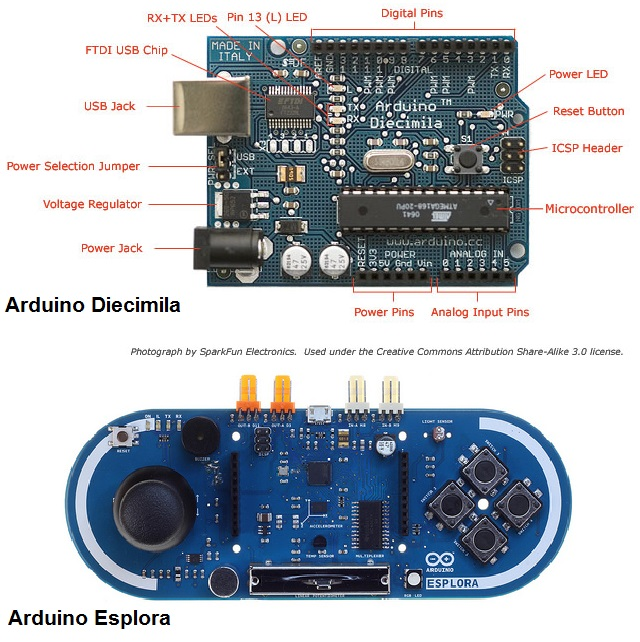
\includegraphics[scale=0.4]{Arduino.jpg}
  \caption{Algunas de las placas de Arduino existentes en el mercado.}
  \label{fig:LegoMindstorms}
\end{figure}

  \item {\bf LEGO Mindstorms}:\footnote{\url{http://mindstorms.LEGO.com/en-us/default.aspx/}} Dentro de las fortalezas de este tipo de sistema, destaca su facilidad de armado y la predefinici\'on de muchos de sus sistemas, adem\'as de la versatilidad de funciones que es capaz de desarrollar. Al mismo tiempo, su alto costo y la restricci\'on del software necesario para desarrollar en \'el se destacan como sus mayores debilidades. Al mismo tiempo posee una baja curva de aprendizaje a la hora de programarlo; sin incluir que no es necesario saber de electr\'onica para su armado.
\begin{figure}[H]
  \centering
  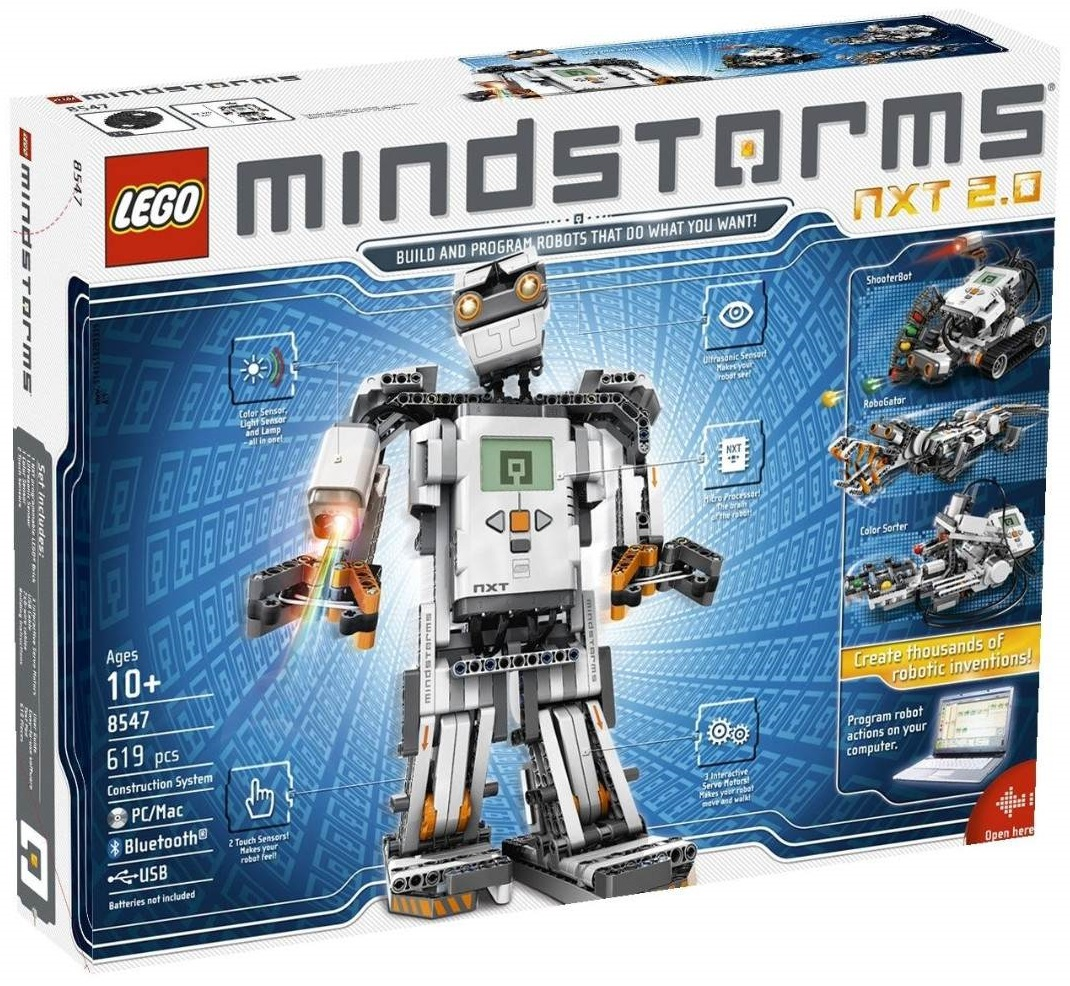
\includegraphics[scale=0.25]{LegoMindstorms.jpg}
  \caption{Box de LEGO Mindstorms.}
  \label{fig:LegoMindstorms}
\end{figure}

  \end{enumerate}
\end{enumerate}

\newpage
\section{Soluci\'on recomendada.}

En base a todo lo expuesto con anterioridad, el enfoque del proyecto que se plantea, corresponde a la uni\'on de dos tecnolog\'ias, es decir, el uso de mascotas tanto en el \'ambito virtual como rob\'otico, permitiendo la interacci\'on del usuario por medio de estas dos plataformas. Para ello, se hace necesario poder identificar las tecnolog\'ias a utilizarse, en base a las restricciones planteadas.

Atendiendo a la restricci\'on n\'umero 5, referente al tiempo de duraci\'on del proyecto, la utilizaci\'on de Arduino o similares queda descartada, debido al alto impacto que tendr\'ia en el tiempo de duraci\'on de este. Dise\~nar y construir un robot con las caracter\'isticas requeridas, en cuanto a sensores, movimiento y comunicaci\'on, requiere una cantidad de tiempo y personal que exceder\'ia las restricciones de tiempo impuestas (ya que adem\'as del robot a utilizar, es necesaria la implementaci\'on del software correspondiente). En vista de ello, se har\'a utilizaci\'on de los robot LEGO Mindstorms, lo que disminuir\'a en gran medida el costo de tiempo para la construcci\'on del modelo rob\'otico, permitiendo adem\'as, una gama amplia de posibles dise\~nos de robots que puedan ser utilizados para el desarrollo del proyecto, debido a su gran versatilidad en la construcci\'on.

En cuanto a la restricci\'on n\'umero 4, esta queda solucionada inmediatamente con la selecci\'on de LEGO Mindstorms, debido a que es posible comunicar los NXT Intelligent Brick\footnote{\url{http://www.mathcs.org/robotics/nxt-java/building/nxt_intro.html/}} por medio de la tecnolog\'ia Bluetooth a los dispositivos m\'oviles. Por lo que no afecta en nada a la selecci\'on del modelo rob\'otico ya planteada. En cuanto al SO a utilizar, esta restricci\'on no ayuda en su determinaci\'on, ya que todos lo dispositivos m\'oviles, en la actualidad, cuentan con Bluetooth.

Respecto a la restricci\'on n\'umero 3, existen librer\'ias para tratar con la compatibilidad entre distintas versiones de los distintos SO existentes en el mercado, por lo que tampoco es determinante en la selecci\'on de la tecnolog\'ia m\'ovil a utilizar.

Finalmente, en respuesta a la restricci\'on n\'umero 2, que impone un bajo costo en el desarrollo del proyecto y en relaci\'on a la restricci\'on n\'umero 1, que habla sobre la facilidad de acceso de los dispositivos m\'oviles, se har\'a uso de SO Android. Lo anterior debido a que corresponde al SO con un mayor mercado en el \'ambito de los dispositivos m\'oviles (en contraste con Windows Mobile o iOS)\footnote{Tendencias de dispositivos moviles para 2013 \url{http://blogthinkbig.com/tendencias-dispositivos-moviles-2013/}} \footnote{Mobile Devices \url{http://www.newmediatrendwatch.com/markets-by-country/17-usa/855-mobile-devices?showall=1}} y, por otro lado, el acceso a desarrollo de aplicaciones no se encuentra limitado a SO determinados (como corresponde al caso iOS, que requiere equipos iMac para su elaboraci\'on, que poseen un costo de adquisici\'on alto).

En vista de lo expuesto con anterioridad, se reafirma el uso de SO Android en los dispositivos m\'oviles a utilizar, adem\'as de LEGO Mindstorms para los robots a dise\~nar durante el desarrollo del proyecto.
 %1. Material Formal
\chapter{T\'ecnicas y herramientas de desarrollo.}
\newpage
%Para el desarrollo de este proyecto, se ha decidido utilizar distintas metodolog\'ias y herramientas, muchas de las cuales son utilizadas dia a dia por miembros del equipo. 

\section{Modelo de desarrollo.}
~\\
Se ha decidido usar el modelo de desarrollo RUP (Rational Unified Process) para la implementaci\'on de este proyecto. RUP es un modelo que promueve el desarrollo iterativo y organiza la elaboraci\'on de software en 4 fases (inicio, elaboraci\'on, desarrollo y cierre) las cuales consisten de una o m\'as iteraciones ejecutables de este. 

\begin{figure}[H]
  \centering
  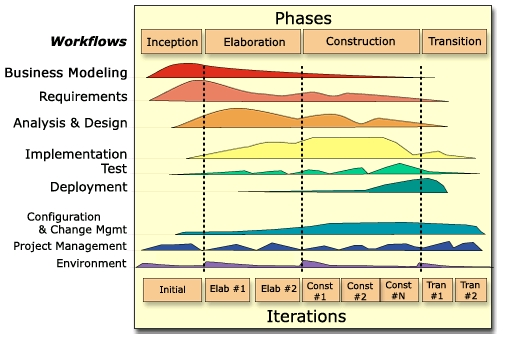
\includegraphics[scale=0.45]{Modelo.jpg}
%  \capture{}
  \label{fig:RUP}
\end{figure}

Este proyecto se separar\'a en cuatro secciones correspondientes a cada una de las entregas de ejecutables, las cuales se profundizar\'an en las cuatro iteraciones del ciclo de desarrollo. Las secciones son:

\begin{enumerate}
\item Funcionamiento b\'asico, dise\~no de robot
\item Implementaci\'on mascota virtual
\item Interacci\'on con robot
\item Interface, fluidez de interacci\'on entre mascota virtual y robot.
\end{enumerate}

De esta forma, se llevar\'an a cabo las distintas etapas de una manera iterativa, secuencial, modularizada e incremental.

Las especificaciones de los casos de uso y requerimientos se encuentran en el archivo Anexo.xlsx

\newpage
\section{Herramientas y t\'ecnicas de soporte para el desarrollo.}
~\\
Para el desarrollo de Viper, el equipo Phyrex ha decidido utilizar las siguientes herramientas:

\begin{itemize}
    \item {\bf Sistema operativo Android 2.1 o superior}: Plataforma oficial de la aplicaci\'on
    \item {\bf Java}: Lenguaje de programaci\'on usado para la aplicaci\'on de Android
    \item {\bf C}: Lenguaje de programaci\'on usado para programar robot LEGO Mindstorms NXT
    \item {\bf UML}: Lenguaje de modelado de base de datos
    \item {\bf Photoshop }: Herramienta de dise\~no gr\'afico
    \item {\bf LEGO Digital Designer}: Herramienta de dise\~no y armado de estructuras de LEGO
    \item {\bf Google docs}: Herramienta de edici\'on colaborativa de documentos
    \item {\bf Git}: Herramienta de control de versiones
    \item {\bf Android SDK tools}: Herramientas de desarrollo en Android
    \item {\bf Eclipse}: Entorno de desarrollo para Android
    \item {\bf SQLite}: Base de datos para la aplicaci\'on
    \item {\bf LEGO Mindstorms NXT}: Robot programable de LEGO
    \item {\bf LEGO Mindstorms 2.0}: Ambiente de desarrollo para Mindstorms
    \item {\bf ROBOTC for LEGO Mindstorms}: Ambiente de desarrollo para Mindstorms
    \item {\bf Skype}: Herramienta de comunicaci\'on entre miembros del equipo
    \item {\bf Facebook}: Herramienta para comunicaci\'on de noticias del proyecto
    \item {\bf \LaTeX}: Edici\'on de documentos
    \item {\bf Microsoft Project}: Herramienta de creaci\'on y manejo de carta gantt
    \item {\bf StarUML}: Herramienta de modelado de casos de uso
    \item {\bf Trello}: Herramienta de gesti\'on de proyectos
\end{itemize}

\newpage
\section{Personal y capacitaci\'on del equipo de desarrollo.}
~\\
Para el desarrollo del proyecto, se necesita contar con un equipo que tenga conocimientos en Java para desarrollo en Android, SQLite, ROBOTC para LEGO Mindstorms, y Photoshop. 

El equipo de desarrollo para este proyecto es la pre-empresa Phyrex, una pre-empresa formada por cinco estudiantes de ingenier\'ia civil inform\'atica de la UTFSM, los cuales se presentan a continuaci\'on:

\begin{itemize}
\item {\bf Juan Avalo}: Experiencia en los lenguajes relevantes (Java, C). 
\item {\bf Celeste Bertin}: Experiencia previa en desarrollo en Android, aprendizaje r\'apido para resolver problemas nuevos. 
\item {\bf Patricio Carrasco}: Programador con experiencia en varios lenguajes.
\item {\bf Roc\'io Fern\'andez}: H\'abil dise\~nadora gr\'afica, experiencia previa en desarrollo en Android, C y librer\'ia gr\'afica AndEngine, uso avanzado de LEGO. 
\item {\bf Rodrigo Fr\'ias}: Experiencia en maquetaci\'on de textos y programaci\'on en C.
\end{itemize}

El equipo esta en constante aprendizaje de Android para sacarle el mayor provecho a esta tecnolog\'ia. El equipo esta en capacitaci\'on de ROBOTC a trav\'es de tutoriales y documentaci\'on disponible en la web. 
 %2. Lecciones
\chapter{Gesti\'on de riesgos}
\newpage
\section{An\'alisis de riesgos}

Los riesgos que han podido ser identificados se detallan a continuaci\'on, indicandose a que tipo pertenecen:

\begin{itemize}
\item {\bf Riesgos T\'ecnicos}:
  \begin{itemize}
  \item[{\bf RT1.}] Errores de inicio y mantenci\'on de conexi\'on v\'ia Bluetooth entre aplicaci\'on y sistema rob\'otico.
  \item[{\bf RT2.}] Problemas de compatibilidad de hardware.
  \item[{\bf RT3.}] Inconsistencia entre robot f\'isico y mascota virtual.
  \item[{\bf RT4.}] P\'erdida de acceso al robot, ya sea por robo o falla t\'ecnica.
  \end{itemize}
\item {\bf Riesgos de Proyecto}:
  \begin{itemize}
  \item[{\bf RP1.}] Falta de experiencia de miembros del equipo en programaci\'on en ROBOTC y Android
  \item[{\bf RP2.}] P\'erdida de personal.
  \item[{\bf RP3.}] Problemas inesperados durante la implementaci\'on del proyecto.
  \item[{\bf RP4.}] Alto costo monetario de hardware o software necesario para la implementaci\'on.
  \end{itemize}
\item {\bf Riesgos de Negocio}:
  \begin{itemize}
  \item[{\bf RN1.}] Cese y desista por parte de LEGO.
  \item[{\bf RN2.}] Aplicaci\'on poco atractiva para p\'ublico objetivo.
  \end{itemize}
\end{itemize}

\section{Preparaci\'on para control de riesgos}

Para poder hacer frente a los riesgos identificados, se detallan a continuaci\'on, indicando la prioridad, impacto, probabilidad, tipo de riesgo, contexto, plan de contingencia y de mitigaci\'on y la resoluci\'on de cada uno de ellos.

La simbolog\'ia asociada a cada detalle es:

\begin{itemize}
\item \emph{Prioridad e Impacto}: entre m\'as cercano a 1 es menor (escala de  1 a  5). 
\item \emph{Probabilidad}: entre m\'as cercano a 1 mayor. (escala de 0 a 1).
\end{itemize}

Se iniciar\'a indicando los riesgos de tipo T\'ecnicos, luego los de Proyecto y finalmente los de Negocio.

\newpage
\subsection{Riesgos T\'ecnicos}

%%
%%Riesgo RT1
%%
\begin{table}[htbp!]
  \centering
  \begin{tabular}{|p{4cm}p{1cm}|p{4cm}p{1cm}|p{4cm}p{1cm}|}\hline
    \multicolumn{2}{|m{5cm}}{\bf Riesgo RT1}& \multicolumn{4}{m{11cm}|}{\justifying Errores de inicio y mantenci\'on de conexi\'on v\'ia Bluetooth entre aplicaci\'on y sistema rob\'otico.}\\\hline
    {\bf Prioridad}& 5& {\bf Impacto}& 5& {\bf Probabilidad}& 0.3\\\hline
    \multicolumn{2}{|m{5cm}}{\bf Tipo de Riesgo}& \multicolumn{4}{m{11cm}|}{\justifying T\'ecnico.}\\\hline
    \multicolumn{2}{|m{5cm}}{\bf Contexto}& \multicolumn{4}{m{11cm}|}{\justifying La interacci\'on de ambos sistemas se da exclusivamente por este medio, lo cual influye de manera considerable en la funcionalidad que se pueda obtener.
Se estima esencial la conexi\'on entre el robot y el smartphone ya que la correlaci\'on de ambas herramientas, as\'i como la fuente de su innovaci\'on, reside en su comunicaci\'on.}\\\hline
    \multicolumn{2}{|m{5cm}}{\bf Plan de Contingencia}& \multicolumn{4}{m{11cm}|}{\justifying El control de este riesgo es fundamental para el proyecto, ya sea lograr una conexi\'on exitosa, como mantenerla durante el tiempo de utilizaci\'on de la aplicaci\'on.\\
En caso de no poder cumplir uno de estos dos requerimientos se deber\'an tomar medidas para mitigar el problema, de no poder reemplazar la conexi\'on, se trabajara solo con uno de los dos aparatos (NXT o Smarthphone) lo que disminuye notablemente la innovaci\'on del proyecto.}\tabularnewline\hline
    \multicolumn{2}{|m{5cm}}{\bf Plan de Mitigaci\'on}& \multicolumn{4}{m{11cm}|}{\justifying De no lograrse una conexi\'on exitosa entre el NXT Intelligent Brick y el smartphone con Android:\begin{enumerate}\item se utilizar\'a un aparato m\'ovil con sistema operativo iOS permitiendo conservar la fuente de innovaci\'on tanto por parte de la interacci\'on entre el dispositivo y el robot, como la utilizaci\'on de sensores del smartphone para variadas funcionalidades.\item Se realizar\'a una conexi\'on v\'ia bluetooth con un computador.\item Se realizar\'a una conexi\'on v\'ia USB con el computador.\end{enumerate}}\\\hline
    \multicolumn{2}{|m{5cm}}{\bf Resoluci\'on}& \multicolumn{4}{m{11cm}|}{\justifying Al conectar exitosamente los dispositivos y mantener la conexi\'on se tendr\'a la base para llevar a cabo todo lo que demanda el proyecto.}\\\hline
  \end{tabular}
  \caption[~RT1]{Control de Riesgo T\'ecnico: RT1}
  \label{table:RT1}
\end{table}


%%
%%Riesgo RT2
%%
\begin{table}[htbp!]
  \centering
  \begin{tabular}{|p{4cm}p{1cm}|p{4cm}p{1cm}|p{4cm}p{1cm}|}\hline
        \multicolumn{2}{|m{5cm}}{\bf Riesgo RT2}& \multicolumn{4}{m{11cm}|}{\justifying Problemas de compatibilidad de hardware.}\\\hline
    {\bf Prioridad}& 3 & {\bf Impacto}& 4 & {\bf Probabilidad}& 0.9\\\hline
    \multicolumn{2}{|m{5cm}}{\bf Tipo de Riesgo}& \multicolumn{4}{m{11cm}|}{\justifying T\'ecnico.}\\\hline
    \multicolumn{2}{|m{5cm}}{\bf Contexto}& \multicolumn{4}{m{11cm}|}{\justifying El hardware del celular no es el esperado, y no presenta todas las caracter\'isticas requeridas para el correcto funcionamiento de la aplicaci\'on, por ejemplo se quiere utilizar el sensor de luz de un smartphone para cierta funci\'on de la aplicaci\'on, pero el Smartphone no lo tiene, por lo que el programa se cae.}\\\hline
    \multicolumn{2}{|m{5cm}}{\bf Plan de Contingencia}& \multicolumn{4}{m{11cm}|}{\justifying Al tratar de utilizar un sensor que no esta presente en el smartphone puede provocar la ca\'ida de la aplicaci\'on, por lo cual esta no ser\'ia compatible con todos los smartphones.\\
Si no se puede detectar la presencia de sensores en el smartphone se utilizaran los m\'as comunes presentes en los smartphone.}\tabularnewline\hline
    \multicolumn{2}{|m{5cm}}{\bf Plan de Mitigaci\'on}& \multicolumn{4}{m{11cm}|}{\justifying De no estar presente alguno de los sensores que se desea utilizar:\begin{enumerate}\item Detectar los sensores presentes en el smartphone  para bloquear o dar opciones acerca de su uso.\item Disminuir el uso de sensores al m\'inimo.\end{enumerate}}\\\hline
    \multicolumn{2}{|m{5cm}}{\bf Resoluci\'on}& \multicolumn{4}{m{11cm}|}{\justifying Al mitigar este riesgo la aplicaci\'on no se caer\'a cuando intente usar sensores del smartphone.}\\\hline
  \end{tabular}
  \caption[~RT2]{Control de Riesgo T\'ecnico: RT2}
  \label{table:RT2}
\end{table}


%%
%%Riesgo RT3
%%
\begin{table}[htbp!]
  \centering
  \begin{tabular}{|p{4cm}p{1cm}|p{4cm}p{1cm}|p{4cm}p{1cm}|}\hline
        \multicolumn{2}{|m{5cm}}{\bf Riesgo RT3}& \multicolumn{4}{m{11cm}|}{\justifying Inconsistencia entre robot f\'isico y mascota virtual.}\\\hline
    {\bf Prioridad}& 4 & {\bf Impacto}& 4 & {\bf Probabilidad}& 0.8\\\hline
    \multicolumn{2}{|m{5cm}}{\bf Tipo de Riesgo}& \multicolumn{4}{m{11cm}|}{\justifying T\'ecnico.}\\\hline
    \multicolumn{2}{|m{5cm}}{\bf Contexto}& \multicolumn{4}{m{11cm}|}{\justifying La arquitectura f\'isica es distinta a la de la figura virtual, por ejemplo la mascota virtual considera tres motores pero el robot f\'isico presenta solo dos, otro caso podr\'ia ser que los motores y sensores est\'an conectados en puertos distintos a los que considera el programa, resultando en el mal funcionamiento del robot y la aplicaci\'on.}\\\hline
    \multicolumn{2}{|m{5cm}}{\bf Plan de Contingencia}& \multicolumn{4}{m{11cm}|}{\justifying Al generar una reacci\'on en el robot por medio de la aplicaci\'on este no reaccionaria de la forma esperada, por ejemplo, se quiere que el robot camine, pero los motores de sus patas no est\'an conectados donde la aplicaci\'on espera, lo que va a resultar en que el perro no pueda caminar correctamente.\\
De darse esto, podr\'ia advertirse al usuario que el robot no se puede modificar, o si lo hace es bajo su propio riesgo.}\tabularnewline\hline
    \multicolumn{2}{|m{5cm}}{\bf Plan de Mitigaci\'on}& \multicolumn{4}{m{11cm}|}{\justifying Para evitar problemas de inconsistencia entre la maqueta f\'isica y virtual de la mascota se puede:\begin{enumerate}\item Crear un wizard de configuraci\'on de los motores, de manera que el usuario pueda modificar el robot sin problemas.\item Crear un mensaje donde se indique la posicion en donde el programa espera que esten conectados los motores.\end{enumerate}}\\\hline
    \multicolumn{2}{|m{5cm}}{\bf Resoluci\'on}& \multicolumn{4}{m{11cm}|}{\justifying Al ejecutar una acci\'on en el robot la cual proviene de la aplicaci\'on este la realizar\'a sin problemas.}\\\hline
  \end{tabular}
  \caption[~RT3]{Control de Riesgo T\'ecnico: RT3}
  \label{table:RT3}
\end{table}


%%
%%Riesgo RT4
%%
\begin{table}[htbp!]
  \centering
  \begin{tabular}{|p{4cm}p{1cm}|p{4cm}p{1cm}|p{4cm}p{1cm}|}\hline
        \multicolumn{2}{|m{5cm}}{\bf Riesgo RT4}& \multicolumn{4}{m{11cm}|}{\justifying P\'erdida de acceso al robot, ya sea por robo o falla t\'ecnica.}\\\hline
    {\bf Prioridad}& 4 & {\bf Impacto}& 5 & {\bf Probabilidad}& 0.3\\\hline
    \multicolumn{2}{|m{5cm}}{\bf Tipo de Riesgo}& \multicolumn{4}{m{11cm}|}{\justifying T\'ecnico.}\\\hline
    \multicolumn{2}{|m{5cm}}{\bf Contexto}& \multicolumn{4}{m{11cm}|}{\justifying Para la realizaci\'on del proyecto es necesaria la utilizaci\'on del NXT Intelligent Brick y componentes de este como motores y sensores, la falla de cualquiera de estos o la p\'erdida de acceso debido a robo pueden causar serios problemas con el avance del proyecto llev\'andolo al fracaso.}\\\hline
    \multicolumn{2}{|m{5cm}}{\bf Plan de Contingencia}& \multicolumn{4}{m{11cm}|}{\justifying Se requiere el robot para la interacci\'on con la aplicaci\'on, sin la presencia de este no se puede avanzar el proyecto o se deber\'a perder gran parte de la innovaci\'on de este.\\
De no tener acceso al robot se deber\'a eliminar toda interacci\'on con este.}\tabularnewline\hline
    \multicolumn{2}{|m{5cm}}{\bf Plan de Mitigaci\'on}& \multicolumn{4}{m{11cm}|}{\justifying En caso de p\'erdida, robo o falla del robot se puede:\begin{enumerate}\item Comprar la pieza que falla.\item Pedir un robot nuevo a la Universidad o Cliente.\item Comprar un kit NXT Intelligent Brick nuevo.\end{enumerate}}\\\hline
    \multicolumn{2}{|m{5cm}}{\bf Resoluci\'on}& \multicolumn{4}{m{11cm}|}{\justifying Si se tiene el robot funcionando $100\%$ se podr\'a avanzar en el proyecto sin retrasos.}\\\hline
  \end{tabular}
  \caption[~RT4]{Control de Riesgo T\'ecnico: RT1}
  \label{table:RT4}
\end{table}

\newpage
\subsection{Riesgos de Proyecto}
%%
%%Riesgo RP1
%%
\begin{table}[htbp!]
  \centering
  \begin{tabular}{|p{4cm}p{1cm}|p{4cm}p{1cm}|p{4cm}p{1cm}|}\hline
        \multicolumn{2}{|m{5cm}}{\bf Riesgo RP1}& \multicolumn{4}{m{11cm}|}{\justifying Falta de experiencia de miembros del equipo en programaci\'on en ROBOTC y Android.}\\\hline
    {\bf Prioridad}& 3 & {\bf Impacto}& 4 & {\bf Probabilidad}& 0.6\\\hline
    \multicolumn{2}{|m{5cm}}{\bf Tipo de Riesgo}& \multicolumn{4}{m{11cm}|}{\justifying Proyecto.}\\\hline
    \multicolumn{2}{|m{5cm}}{\bf Contexto}& \multicolumn{4}{m{11cm}|}{\justifying Este proyecto requiere programaci\'on en Android SDK el cual trabaja con Java, y para el NXT Intelligent Brick ROBOTC, por esta raz\'on es necesario tener conocimientos de estos lenguajes, para el correcto avance del proyecto.}\\\hline
    \multicolumn{2}{|m{5cm}}{\bf Plan de Contingencia}& \multicolumn{4}{m{11cm}|}{\justifying Si gran parte de los miembros del equipo de trabajo no cuentan con conocimientos en los lenguajes que se requiere utilizar, esto puede a llevar a que el proyecto falle.\\
Por esto como medida de emergencia se recargar\'a a los miembros del equipo con m\'as conocimiento en los lenguajes a utilizar.}\tabularnewline\hline
    \multicolumn{2}{|m{5cm}}{\bf Plan de Mitigaci\'on}& \multicolumn{4}{m{11cm}|}{\justifying En caso de que los miembros del equipo no cuenten con suficiente conocimiento y experiencia se puede:\begin{enumerate}\item Capacitar a los miembros del equipo con menos conocimientos recibiendo clases de parte de los miembros con m\'as conocimientos.\item Utilizar la documentaci\'on disponible en internet como herramienta de autoaprendizaje.\end{enumerate}}\\\hline
    \multicolumn{2}{|m{5cm}}{\bf Resoluci\'on}& \multicolumn{4}{m{11cm}|}{\justifying Si los miembros del equipo tiene conocimiento y experiencia con los lenguajes que se requiere utilizar disminuyen dr\'asticamente las probabilidades de que el proyecto falle.}\\\hline
  \end{tabular}
  \caption[~RP1]{Control de Riesgo T\'ecnico: RP1}
  \label{table:RP1}
\end{table}


%%
%%Riesgo RP2
%%
\begin{table}[htbp!]
  \centering
  \begin{tabular}{|p{4cm}p{1cm}|p{4cm}p{1cm}|p{4cm}p{1cm}|}\hline
        \multicolumn{2}{|m{5cm}}{\bf Riesgo RP2}& \multicolumn{4}{m{11cm}|}{\justifying P\'erdida de personal.}\\\hline
    {\bf Prioridad}& 2 & {\bf Impacto}& 4 & {\bf Probabilidad}& 0.9\\\hline
    \multicolumn{2}{|m{5cm}}{\bf Tipo de Riesgo}& \multicolumn{4}{m{11cm}|}{\justifying Proyecto.}\\\hline
    \multicolumn{2}{|m{5cm}}{\bf Contexto}& \multicolumn{4}{m{11cm}|}{\justifying El equipo cuenta con 5 miembros los cuales se dividen el trabajo para avanzar en el proyecto, y presentar las entregas en las fechas requeridas. El tama\~no del equipo es adecuado para el trabajo que debe realizarse, pero pueden ocurrir casos donde uno o m\'as miembros no puedan colaborar con el trabajo ya se a  causa de una enfermedad, problemas personales que generen poca disponibilidad o falta de tiempo a causa de otros ramos.}\\\hline
    \multicolumn{2}{|m{5cm}}{\bf Plan de Contingencia}& \multicolumn{4}{m{11cm}|}{\justifying Se deben realizar entregas peri\'odicas de avance, ya sean informes como avance de la aplicaci\'on, por lo que se debe trabajar en conjunto para tener las entregas listas en la fecha que se requiere.\\
En el caso de que alg\'un miembro no pueda realizar el trabajo que se le hab\'ia asignado el equipo se ver\'a en la obligaci\'on de repartir su parte entre los miembros restantes.}\tabularnewline\hline
    \multicolumn{2}{|m{5cm}}{\bf Plan de Mitigaci\'on}& \multicolumn{4}{m{11cm}|}{\justifying Si uno o m\'as de los miembros de equipo no puede realizar su trabajo se puede:\begin{enumerate}\item En caso de que los miembros no puedan tener disponibilidad debido a pruebas de otros ramos se puede realizar un calendario con todas las evaluaciones y as\'i poder programar c\'omo y cu\'ando se trabajar\'a.\item En caso de enfermedad, se puede disminuir la carga de trabajo del individuo enfermo o redistribuir los trabajos para, en caso de que se pueda, permitir que trabaje desde su hogar.\item En caso de p\'erdida definitiva se disminuir\'a el alcance del proyecto.\end{enumerate}Cabe destacar que ya ha sido necesario realizar, debido a que Patricio Carrasco no continuar\'a en el equipo el pr\'oximo semestre, por lo que se redujo la carga de cada entrega para disminuir la cantidad de trabajo de los miembros restantes del equipo en los pr\'oximos entregables.}\\\hline
    \multicolumn{2}{|m{5cm}}{\bf Resoluci\'on}& \multicolumn{4}{m{11cm}|}{\justifying Al tener disponibilidad de todo el personal de trabajo no solo existe una mayor probabilidad de entregar en la fecha adecuada, sino que tambi\'en se disminuye la carga de todos.}\\\hline
  \end{tabular}
  \caption[~RP2]{Control de Riesgo T\'ecnico: RP2}
  \label{table:RP2}
\end{table}


%%
%%Riesgo RP3
%%
\begin{table}[htbp!]
  \centering
  \begin{tabular}{|p{4cm}p{1cm}|p{4cm}p{1cm}|p{4cm}p{1cm}|}\hline
        \multicolumn{2}{|m{5cm}}{\bf Riesgo RP3}& \multicolumn{4}{m{11cm}|}{\justifying Problemas inesperados durante la implementaci\'on del proyecto.}\\\hline
    {\bf Prioridad}& 3 & {\bf Impacto}& 2 & {\bf Probabilidad}& 0.2\\\hline
    \multicolumn{2}{|m{5cm}}{\bf Tipo de Riesgo}& \multicolumn{4}{m{11cm}|}{\justifying Proyecto.}\\\hline
    \multicolumn{2}{|m{5cm}}{\bf Contexto}& \multicolumn{4}{m{11cm}|}{\justifying Al ser un proyecto en el cual se trabaja con herramientas nuevas, siempre existe la posibilidad de tener problemas inesperados en su transcurso, los cuales pueden afectar directamente su probabilidad de \'exito.\\
En el caso de que ocurran problemas inesperados que consuman tiempo extra no esperado al trabajar, por ejemplo, con  Android y ROBOTC.}\tabularnewline\hline
    \multicolumn{2}{|m{5cm}}{\bf Plan de Contingencia}& \multicolumn{4}{m{11cm}|}{\justifying Si llegasen a ocurrir errores al trabajar con Android, ROBOTC o alguna de las herramientas que se requieren usar y consuman demasiado tiempo afectando el avance en las entregas se  deber\'a encontrar la medida de contingencia adecuada, siendo la persona m\'as experimentada en el \'area del problema la encargada de dirigir el proceso. El resto del equipo validar\'a e implementar\'a la soluci\'on una vez encontrada.}\\\hline
    \multicolumn{2}{|m{5cm}}{\bf Plan de Mitigaci\'on}& \multicolumn{4}{m{11cm}|}{\justifying En caso de que problemas inesperados ocurran durante la implementaci\'on  del proyecto se puede:\begin{enumerate}\item Organiza el calendario de tal forma de dejar un margen entre la fecha de entrega y la finalizaci\'on de \'esta, para as\'i evitar casos de falta de tiempo por problemas inesperados.\item Volver a repartir el trabajo entre el equipo para ayudar a quien se vea afectado por el problema.\end{enumerate}}\\\hline
    \multicolumn{2}{|m{5cm}}{\bf Resoluci\'on}& \multicolumn{4}{m{11cm}|}{\justifying Si se pueden prevenir los problemas inesperados, se evitar\'an problemas de falta de tiempo al realizar las entregas.}\\\hline
  \end{tabular}
  \caption[~RP3]{Control de Riesgo T\'ecnico: RP3}
  \label{table:RP3}
\end{table}


%%
%%Riesgo RP4
%%
\begin{table}[htbp!]
  \centering
  \begin{tabular}{|p{4cm}p{1cm}|p{4cm}p{1cm}|p{4cm}p{1cm}|}\hline
        \multicolumn{2}{|m{5cm}}{\bf Riesgo RP4}& \multicolumn{4}{m{11cm}|}{\justifying Alto costo monetario de hardware o software necesario para la implementaci\'on.}\\\hline
    {\bf Prioridad}& 3 & {\bf Impacto}& 3 & {\bf Probabilidad}& 0.5\\\hline
    \multicolumn{2}{|m{5cm}}{\bf Tipo de Riesgo}& \multicolumn{4}{m{11cm}|}{\justifying Proyecto.}\\\hline
    \multicolumn{2}{|m{5cm}}{\bf Contexto}& \multicolumn{4}{m{11cm}|}{\justifying Se trabajar\'a con smartphones y LEGO Mindstorms para la realizaci\'on del proyecto, por lo que se pueden requerir componentes que no estaban presupuestados o tengan un valor mayor  al esperado, por ejemplo, sensores o piezas para el robot.\\
Adem\'as se requiere licencias para software, por ejemplo, ROBOTC.}\tabularnewline\hline
    \multicolumn{2}{|m{5cm}}{\bf Plan de Contingencia}& \multicolumn{4}{m{11cm}|}{\justifying Dado que muchos de los elementos requeridos para el proyecto, ya sea hardware o software conllevan un costo, es probable que est\'en fuera del presupuesto esperado, lo cual afectar\'ia directamente en el proyecto.\\
En caso de no poder costear alguno de los elementos necesarios se deber\'a obviar su uso, esto dependiendo de qu\'e tan esencial sea para el \'exito del proyecto.}\tabularnewline\hline
    \multicolumn{2}{|m{5cm}}{\bf Plan de Mitigaci\'on}& \multicolumn{4}{m{11cm}|}{\justifying De no contar con presupuesto para tener acceso a hardware o software necesario se puede:\begin{enumerate}\item Solicitar al cliente que cubra los gastos necesarios.\item Preparar un saldo de emergencia para casos como este.\end{enumerate}}\\\hline
    \multicolumn{2}{|m{5cm}}{\bf Resoluci\'on}& \multicolumn{4}{m{11cm}|}{\justifying Al tener acceso a todos los elementos necesario, ya sean hardware o software disminuir\'a las probabilidades de fallo del proyecto.}\\\hline
  \end{tabular}
  \caption[~RP4]{Control de Riesgo T\'ecnico: RP4}
  \label{table:RP4}
\end{table}

\newpage
\subsection{Riesgos de Negocio}
%%
%%Riesgo RN1
%%
\begin{table}[htbp!]
  \centering
  \begin{tabular}{|p{4cm}p{1cm}|p{4cm}p{1cm}|p{4cm}p{1cm}|}\hline
        \multicolumn{2}{|m{5cm}}{\bf Riesgo RN1}& \multicolumn{4}{m{11cm}|}{\justifying Cese y desista por parte de LEGO.}\\\hline
    {\bf Prioridad}& 1 & {\bf Impacto}& 5 & {\bf Probabilidad}& 0.1\\\hline
    \multicolumn{2}{|m{5cm}}{\bf Tipo de Riesgo}& \multicolumn{4}{m{11cm}|}{\justifying Negocio.}\\\hline
    \multicolumn{2}{|m{5cm}}{\bf Contexto}& \multicolumn{4}{m{11cm}|}{\justifying Para la realizaci\'on del proyecto  se utilizar\'a LEGO Mindstorms para el dise\~no del robot con el cual la aplicaci\'on va a interactuar, por lo cual es importante cumplir con todos los t\'erminos y condiciones de este para as\'i no tener problemas de tipo legales con la empresa.}\\\hline
    \multicolumn{2}{|m{5cm}}{\bf Plan de Contingencia}& \multicolumn{4}{m{11cm}|}{\justifying En el caso de que LEGO denegar\'a los permisos para utilizar LEGO Mindstorms por cualquier incumplimiento de los t\'erminos y condiciones de uso, esto afectar\'ia una parte importante del proyecto quitando gran parte de la innovaci\'on de este, y en el peor caso obligar\'ia a cancelar este.}\\\hline
    \multicolumn{2}{|m{5cm}}{\bf Plan de Mitigaci\'on}& \multicolumn{4}{m{11cm}|}{\justifying En caso de no tener permisos para utilizar LEGO Mindstorms se puede:\begin{enumerate}\item Crear el robot con otro tipo de tecnolog\'ias, por ejemplo, Arduino.\end{enumerate}}\\\hline
    \multicolumn{2}{|m{5cm}}{\bf Resoluci\'on}& \multicolumn{4}{m{11cm}|}{\justifying Si se tiene permisos para utilizar LEGO Mindstorms para el dise\~no del robot se podr\'a seguir contando con la innovaci\'on del negocio.}\\\hline
  \end{tabular}
  \caption[~RN1]{Control de Riesgo T\'ecnico: RN1}
  \label{table:RN1}
\end{table}



%%
%%Riesgo RN2
%%
\begin{table}[htbp!]
  \centering
  \begin{tabular}{|p{4cm}p{1cm}|p{4cm}p{1cm}|p{4cm}p{1cm}|}\hline
        \multicolumn{2}{|m{5cm}}{\bf Riesgo RN2}& \multicolumn{4}{m{11cm}|}{\justifying Aplicaci\'on poco atractiva para p\'ublico objetivo.}\\\hline
    {\bf Prioridad}& 1 & {\bf Impacto}& 2 & {\bf Probabilidad}& 0.9\\\hline
    \multicolumn{2}{|m{5cm}}{\bf Tipo de Riesgo}& \multicolumn{4}{m{11cm}|}{\justifying Negocio.}\\\hline
    \multicolumn{2}{|m{5cm}}{\bf Contexto}& \multicolumn{4}{m{11cm}|}{\justifying La aplicaci\'on esta enfocada a escolares de ense\~nanza media, por lo que esta debe ser atractiva, para as\'i poder cumplir con el objetivo de acercarlos a la inform\'atica.\\
Por esto la aplicaci\'on debe poder atraer la atenci\'on los usuarios como as\'i tambi\'en lograr generar un inter\'es en la inform\'atica.}\tabularnewline\hline
    \multicolumn{2}{|m{5cm}}{\bf Plan de Contingencia}& \multicolumn{4}{m{11cm}|}{\justifying Al tratarse de una aplicaci\'on que tiene como p\'ublico objetivo adolescentes, esta adem\'as de tener una apariencia agradable para ellos debe entretenerlos, si esto no se logra har\'a m\'as dif\'icil cumplir el objetivo de la aplicaci\'on.\\
En el  caso de que la interfaz y caracter\'isticas de la aplicaci\'on no sean atractivas para el p\'ublico objetivo se deber\'a en base a encuestas y pruebas con usuarios trabajar sobre las caracter\'isticas actuales aunque esto implique cambiar gran parte de la aplicaci\'on y su funcionamiento.}\\\hline
    \multicolumn{2}{|m{5cm}}{\bf Plan de Mitigaci\'on}& \multicolumn{4}{m{11cm}|}{\justifying En caso de que la aplicaci\'on no resulte atractiva para el p\'ublico objetivo se puede:\begin{enumerate}\item Realizar un testing con un grupo de estudiantes y obtener datos.\item Realizar encuestas a un grupo de usuarios objetivos.\end{enumerate}}\\\hline
    \multicolumn{2}{|m{5cm}}{\bf Resoluci\'on}& \multicolumn{4}{m{11cm}|}{\justifying Al tener una aplicaci\'on atractiva para los estudiantes se podr\'a cumplir m\'as f\'acilmente el objetivo del negocio.}\\\hline
  \end{tabular}
  \caption[~~RN2]{Control de Riesgo T\'ecnico: RN1}
  \label{table:RN2}
\end{table}
 %3. Sugerencias
\chapter{Material detallado de apoyo}

\section{Roles y actividades en el equipo} %distribucion de los roles y actividades que cada integrante del equipo desempe~o durante el proyecto

\section{Roles y actividades en el equipo} %referencias bibliograficsa, url's, papers y otros en un formato que permita a otros encontrar los recursos citados
 %4. Material Detallado de Apoyo
\part{Parte Privada}              %% Parte Privada
\chapter{Planificaci\'on de actividades.}
\newpage
 %5. Aspectos Mejorables
\chapter{Comentarios Adicionales}

%si hay algun comentario o aporte que el equipo desea hacer dirigido solo a los profesores de los cursos y que no sera publicado en el futuro, debe hacerlo en esta seccion.
 %6. Comentarios Adicionales
%\appendix
\clearpage
\addappheadtotoc
\appendixpage

\chapter{Planificaci\'on de Actividades}
\label{appen:planificacion}

\newpage
\section[WBS]{Work Breakdown Structure}
\label{section:wbs}

En las siguientes p\'aginas se muestra la estimaci\'on del esfuerzo estimado para el proyecto \emph{V.I.Pe.R.}:

\begin{table}[H]
  \centering
  \begin{tabular}{|l|m{5cm}|c|c|c|}\hline
    {\bf Fase} & {\bf Tarea} & {\bf Esfuerzo} & {\bf Hrs. Equipo} & {\bf Hrs. Hombre}\\\hline
    \multirow{4}{*}{Inicio} & Decisi\'on aplicaci\'on                & 3 & 12 & 48\\\cline{2-5}
           & Pruebas de robot                   & 3 & 12 & 48\\\cline{2-5}
           & Definici\'on software de desarrollo  & 2 & 12 & 48\\\cline{2-5}
           & Definici\'on nombre pre-empresa y producto & 2 & 8 & 32\\\hline
    \multirow{7}{*}{Elaboraci\'on} & Propuesta T\'ecnica           & 3 & 12 & 48\\\cline{2-5}
                & Toma de requisitos          & 5 & 20 & 80\\\cline{2-5}
                & Especificaci\'on casos de uso & 4 & 16 & 64\\\cline{2-5}
                & Identificaci\'on de riesgos   & 5 & 20 & 80\\\cline{2-5}
                & Mitigaci\'on de riesgos       & 5 & 20 & 80\\\cline{2-5}
                & P\'agina web                  & 3 & 12 & 48\\\cline{2-5}
                & Plan de proyecto            & 4 & 16 & 64\\\hline
    \multirow{5}{*}{Desarrollo} & Dise\~no de Interfaz                            & 5 & 20 & 100\\\cline{2-5}
               & Programaci\'on de Casos de Uso/Requerimientos   & 5 & 20 & 100\\\cline{2-5}
               & Testing                                       & 3 & 12 & 60\\\cline{2-5}
               & Feedback                                      & 3 & 12 & 60\\\cline{2-5}
               & Algo de nivel 3?!                             &   &    &\\\hline
                & {\bf Total}                 & 55 & 224 & 960\\\hline
  \end{tabular}
  \label{tab:wbs}
  \caption[Tabla WBS]{Divisi\'on de trabajo, seg\'un modelo utilizado, por esfuerzo.}
\end{table}

\newpage
%\section{Carta Gantt}

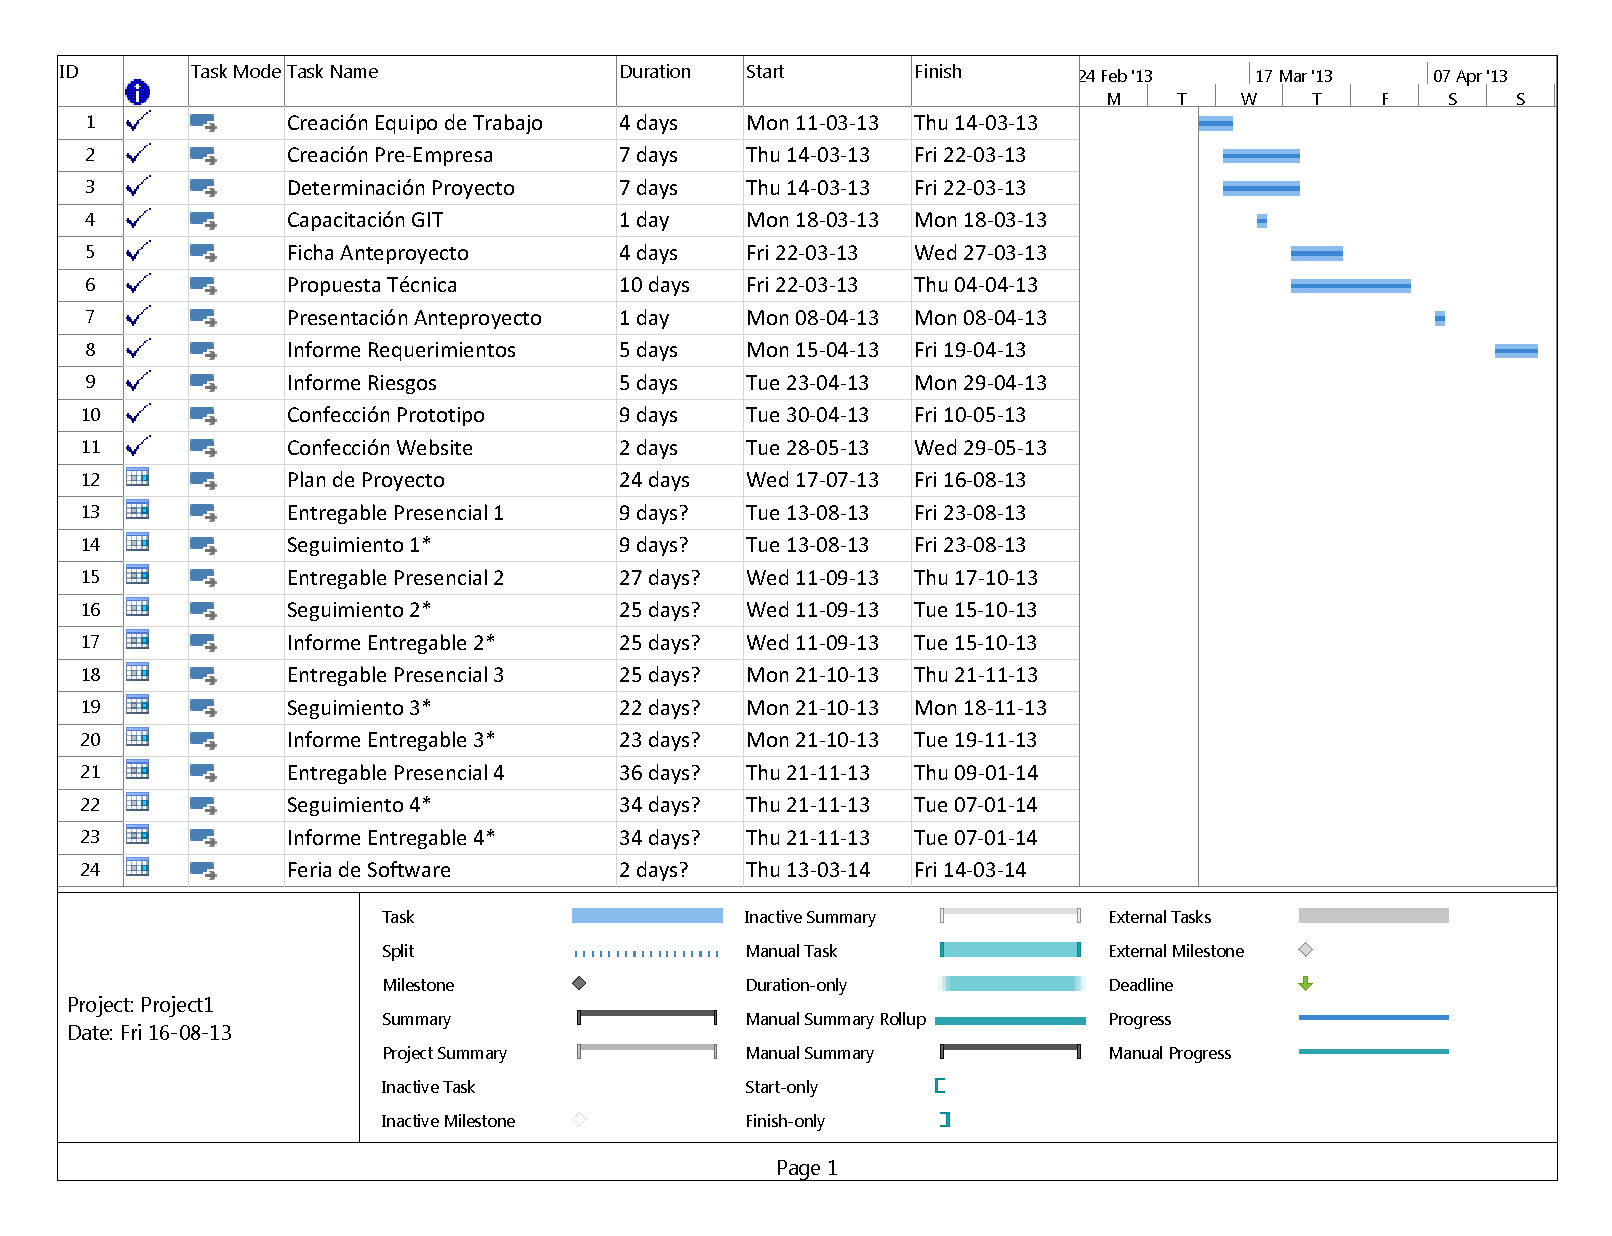
\includepdf[scale=0.7,pages=1,angle=-90,pagecommand=\section{Carta Gantt.}]{./pic/gantt.pdf}
\includepdf[scale=0.7,pages=2-,angle=-90,pagecommand={}]{./pic/gantt.pdf}
%\chapter{Glosario de T\'erminos.}
%\begin{itemize}
%\item {\bf SO}: Abreviatura de \textbf{S}istema \textbf{O}perativo. Programa encargado de la gesti\'on de recursos de Hardware. Provee los servicios a los programas de aplicaci\'on.
%\item LEGO Mindstorms: Juego de rob\'otica para ni\~nos, elaborado por la empresa LEGO en colaboraci\'on con el MIT. Posee distintos tipos de sensores, as\'i como un
%\end{itemize}

%
%
%%Bibliografia
%\backmatter
%\addcontentsline{toc}{chapter}{Bibliograf\'ia}
%\bibliographystyle{acm}
%

\end{document}
